\documentclass[sp,article]{FEIstyle}
\usepackage{tikz}
\usetikzlibrary{arrows.meta,positioning,calc,fit,babel}
\usepackage{float}
\usepackage{placeins}
\usepackage{array}
\addbibresource{referat/bibliography.bib}
\DeclareFieldFormat{doi}{\mkbibacro{DOI}\addcolon\space\href{https://doi.org/#1}{\mbox{\nolinkurl{#1}}}}
\hypersetup{pdftitle={Predikcia výnosov akcií pomocou udalostí a jazykových modelov},pdfauthor={Ilia Liubotin}}
\emergencystretch=1.5em
\captionsetup{font=small,labelfont=bf}
\newcommand{\serref}[1]{\cite[#1]{li2025ser}}
\newcommand{\mentorref}[1]{\cite[#1]{chen2025mentor}}
\newcolumntype{Y}{>{\raggedright\arraybackslash}X}
\tikzset{box/.style={draw=black!65,rounded corners=2pt,fill=black!3,align=center,font=\small,inner sep=6pt},arr/.style={-{Latex[length=2mm]},thick},note/.style={font=\footnotesize,align=center}}
\begin{document}
\begin{titlepage}
\centering
{\large Slovenská technická univerzita v Bratislave\par}
{\large Fakulta elektrotechniky a informatiky\par}
\vspace{3cm}
{\LARGE\bfseries Predikcia výnosov akcií pomocou udalostí a jazykových modelov\par}
\vspace{1.2cm}
{\large Priebežná písomná práca\par}
{\large Bakalársky projekt 1\par}
\vfill
\begin{tabular}{@{}ll@{}}
Študent: & Ilia Liubotin\\
Vedúci práce: & prof. Dr. rer. nat. Martin Drozda
\end{tabular}
\vspace{2cm}
\par Bratislava, november 2026
\end{titlepage}
\section{Úvod}
Správy môžu pomôcť pri odhade budúceho výnosu akcie. Jazykový model ich dokáže spracovať. Najprv však treba určiť jeho úlohu. Opis udalosti, ktorá sa už stala, nie je to isté ako opis možnej budúcej udalosti. Pravdepodobnosť udalosti tiež nie je očakávaný výnos akcie.

V tejto práci opisujem metódu \emph{Structured Event Representation} (SER) autorov Li, Qiao a Zheng. Táto metóda získava udalosti z novinových článkov a používa ich na predikciu výnosov akcií \serref{kap.~2}. Venujem sa jej vstupom, častiam modelu, učeniu a výsledkom. Potom ju porovnávam s metódou MENTOR autorov Chen a kol. MENTOR predikuje budúce udalosti a poradie odvetvových indexov \mentorref{kap.~3--4}.

Na konci uvádzam návrh pre svoju bakalársku prácu. Chcem skúmať predikciu výnosov pred tým, ako sa očakávaná udalosť stane. Vlastný experiment zatiaľ nebol vykonaný.

\section{SER: úloha a údaje}
SER dostáva udalosti spojené s konkrétnou akciou za určité obdobie. Jeho úlohou je odhadnúť výnos tejto akcie v ďalšom období. Autori skúmajú dva prípady: ďalší obchodný deň a ďalší týždeň. Výstupom je číslo, preto ide o regresnú úlohu.

Akciu označíme indexom $i$ a obdobie indexom $t$. Symbol $E_{i,t}$ znamená súbor udalostí pre túto akciu a obdobie. Symbol $s_i$ označuje identifikátor akcie. Model môžeme zapísať podľa rovnice~(1) pôvodného článku takto:
\begin{equation}
\widehat r_{i,t+1}=f_{\theta}(E_{i,t},s_i).
\label{eq:task}
\end{equation}
Symbol $\widehat r_{i,t+1}$ je predikovaný výnos a $\theta$ sú parametre, ktoré sa model učí. Pri učení sa predikcia porovnáva so skutočným výnosom. Znamienko ukazuje, či model očakáva kladný alebo záporný výnos. Toto číslo však nie je pravdepodobnosťou rastu \serref{kap.~2.2.1 a 2.2.4}.

Autori získali výnosy akcií z databázy CRSP. Novinové články pochádzajú z ProQuest a Factiva. Hlavný experiment používa údaje z rokov 2003--2022. Po spracovaní zostalo 301\,409 príkladov typu firma--deň a 4\,355 akcií. Jeden taký príklad spája jednu firmu s jedným dňom. Týždenný výnos sa počíta z denných výnosov podľa vzťahu $r_{\text{týždeň}}=\prod_d(1+r_d)-1$. Súčin zahŕňa platné obchodné dni daného týždňa \serref{kap.~3.1, rovnica~(13)}.

Článok sa najprv priradí ku konkrétnej firme. Systém hľadá jej názov v texte a porovnáva aj podobné zápisy názvu. Ide o približné porovnávanie textov, po anglicky \emph{fuzzy matching}. Názov firmy sa musí objaviť aspoň dvakrát. Vyberie sa firma s najlepšou zhodou. Firmy s nejasnými názvami sa vylúčia. Udalosti z priradených článkov sa potom spoja podľa firmy a dátumu \serref{kap.~3.1; príloha OA.1.3}.

Predikčný model navyše používa číselný vektor identifikátora akcie. Tento vektor sa učí spolu s modelom. Pomáha rozlišovať firmy, pretože rovnaká udalosť môže mať pre rôzne firmy odlišný význam. Priradenie článku firme a učenie tohto vektora sú teda dva rôzne kroky. Tento postup sám nevyhľadáva všetky firmy, na ktoré môže udalosť nepriamo pôsobiť \serref{kap.~2.2.1}.

Články z obdobia $t$ sa spájajú s výnosom v období $t+1$. Pri vlastnom experimente však bude dôležitý aj presný čas. Treba vedieť, kedy správa vyšla, kedy ju systém spracoval a kedy bolo možné vykonať obchod. Samotný dátum správy nestačí na overenie ceny, za ktorú sa dalo reálne vstúpiť do pozície.

\section{SER: získanie udalostí z textu}
\subsection{Čo robí jazykový model}
SER používa hotový veľký jazykový model, označovaný skratkou LLM. Autori zvolili \texttt{gpt-3.5-turbo-0125}. Model číta článok a vyberá z neho udalosti. Každú udalosť zapisuje ako trojicu \emph{subjekt--akcia--objekt}. Subjekt označuje, kto alebo čo vykonáva činnosť. Akcia opisuje túto činnosť a objekt označuje, čoho sa týka. Slovo akcia tu znamená činnosť, nie akciu obchodovanú na burze. LLM v tomto kroku nepredikuje výnos \serref{kap.~2.1 a 3.1}.

Záznam má šesť polí. Základnú trojicu tvoria \texttt{subject}, \texttt{action} a \texttt{object}. Polia \texttt{subject\_link} a \texttt{object\_link} obsahujú odkazy na entity. Pole \texttt{context} obsahuje časť pôvodného textu, ktorá pomáha overiť význam udalosti. Základom vstupu do prediktora zostáva trojica \serref{kap.~2.1; príloha OA.2}.

Pokyn pre LLM určuje formát JSON a obsahuje príklady správnych odpovedí. Model používa tieto príklady pri spracovaní zadania. Jeho váhy sa tým nemenia. Odkazy na databázu DBpedia pomáhajú spojiť rôzne názvy tej istej osoby, firmy alebo inej entity. Entita je tu pomenovaný prvok udalosti. Ak sa jedna firma v textoch objaví pod viacerými názvami, mala by dostať rovnaký identifikátor \serref{kap.~2.1}.

Výsledok kontroluje ďalšie použitie LLM v úlohe hodnotiteľa. Kontroluje formát, potrebné polia a súlad s pôvodným textom. Chybný záznam sa opraví alebo vytvorí znovu. Ak ani po viacerých pokusoch neprejde kontrolou, systém ho vyradí. Autori tiež ručne porovnali náhodne vybrané skupiny výsledkov s pôvodnými článkami \serref{kap.~2.1 a 3.1}. Takáto kontrola pomáha nájsť chyby. Neznamená však, že všetky získané udalosti sú správne. Chyba v udalosti môže neskôr ovplyvniť aj odhad výnosu.

\subsection{Ako sa z udalostí stanú čísla}
Najprv sa odstránia opakované udalosti v tom istom príklade. Slová opisujúce činnosti sa prevedú na základný tvar. Tento krok sa volá lematizácia. Potom sa pomocou BERT prevedú na vektory, teda zoznamy čísel. Algoritmus DBSCAN ich rozdelí do skupín podobných výrazov. Podobné zápisy činností sa tak zjednotia. Subjekty a objekty dostanú identifikátory podľa odkazov DBpedia. Činnosti dostanú vlastné identifikátory \serref{príloha OA.1.4}.

V prediktore má každý identifikátor svoj učený vektor. Takýto vektor sa nazýva \emph{embedding}. Má $M$ čísel a počas učenia sa mení. Vektor celej udalosti vzniká podľa vzťahu
\begin{equation}
z_e=e_{\mathrm{subjekt}}+e_{\mathrm{akcia}}-e_{\mathrm{objekt}}
\in\mathbb{R}^{M}.
\label{eq:event}
\end{equation}
Autori tento postup spájajú s metódou TransE. Vektory subjektu a činnosti sa sčítajú a vektor objektu sa odčíta. Výsledkom je jeden vektor udalosti. Subjekt a objekt tu majú odlišné úlohy. Rovnaké entity môžu používať tie isté učené parametre vo viacerých udalostiach \serref{kap.~2.2.2, rovnica~(2)}.

Článok vysvetľuje TransE pomocou vzťahu, pri ktorom sa súčet vektorov subjektu a činnosti približuje k vektoru objektu. Pre predikciu však používa priamo rozdiel z rovnice~\eqref{eq:event}. Pri opise učenia autori uvádzajú minimalizáciu chyby výnosu. Samostatnú stratovú funkciu pre TransE preto do opisu nepridávam, pretože nie je v tejto časti článku potvrdená \serref{kap.~2.2.2 a 2.2.5}.

Aj identifikátor burzovej akcie má učený vektor $z_i\in\mathbb{R}^{M}$. Model si ho vytvára z tréningových príkladov. Tento vektor nie je zoznamom priamo zadaných údajov o firme, napríklad jej cien alebo zisku. Vektory udalostí a akcií sa učia pre spoločný cieľ: lepšie odhadnúť ďalší výnos.

\section{SER: ako model predikuje výnos}
\subsection{Spojenie udalostí pomocou attention}
K jednej firme môže v jeden deň patriť viac udalostí. Nie všetky musia byť rovnako dôležité. Model ich preto spája pomocou mechanizmu \emph{attention}, teda mechanizmu pozornosti. Tento mechanizmus pracuje s vektormi udalostí a s vektorom akcie. Schému modelu ukazuje obrázok~\ref{fig:ser}.

Na začiatok vstupu sa pridá špeciálny učený vektor $z_{\mathrm{CLS}}$. Jeho úlohou je zhrnúť informácie z ostatných vstupov. Vektory sa uložia do riadkov jednej matice:
\begin{equation}
Z^{(0)}_{i,t}=[z_{\mathrm{CLS}};z_{e_1};\ldots;z_{e_N};z_i]
\in\mathbb{R}^{(N+2)\times M}.
\label{eq:input}
\end{equation}
Matica má $N+2$ riadkov: $N$ udalostí, jeden vektor CLS a jeden vektor akcie. Každý riadok má $M$ čísel. CLS neobsahuje novú správu z trhu. Počas učenia sa naučí zbierať informácie z ostatných riadkov \serref{kap.~2.2.3, rovnica~(3)}.

\begin{figure}[htbp]
\centering
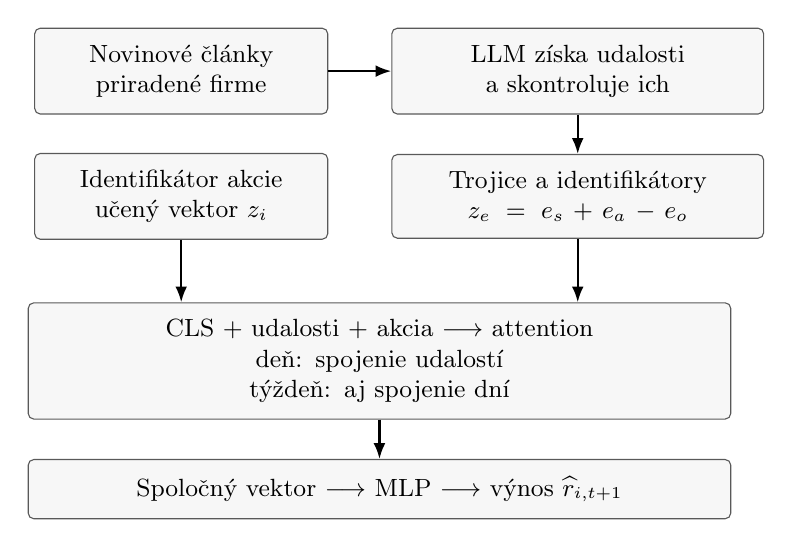
\begin{tikzpicture}[node distance=5mm and 8mm]
\node[box,text width=3.3cm] (news) {Novinové články\\priradené firme};
\node[box,text width=4.3cm,right=of news] (llm) {LLM získa udalosti\\a skontroluje ich};
\node[box,text width=4.3cm,below=of llm] (events) {Trojice a identifikátory\\$z_e=e_s+e_a-e_o$};
\node[box,text width=3.3cm,left=of events] (stock) {Identifikátor akcie\\učený vektor $z_i$};
\node[box,text width=8.5cm,below=8mm of $(events.south)!0.5!(stock.south)$] (att) {CLS + udalosti + akcia $\longrightarrow$ attention\\deň: spojenie udalostí\\týždeň: aj spojenie dní};
\node[box,text width=8.5cm,below=of att] (mlp) {Spoločný vektor $\longrightarrow$ MLP $\longrightarrow$ výnos $\widehat r_{i,t+1}$};
\draw[arr] (news)--(llm);
\draw[arr] (llm)--(events);
\draw[arr] (events.south)--(att.north -| events.south);
\draw[arr] (stock.south)--(att.north -| stock.south);
\draw[arr] (att)--(mlp);
\end{tikzpicture}
\caption{Postup v SER. Vektory a prediktor sa učia podľa ďalších skutočných výnosov. Váhy LLM sa pri tomto učení nemenia. Vlastné spracovanie podľa \serref{kap.~2, obr.~1--3}.}
\label{fig:ser}
\end{figure}


Attention vytvorí zo vstupnej matice $Z$ tri nové matice: $Q=ZW_Q$, $K=ZW_K$ a $V=ZW_V$. Matice $W_Q$, $W_K$ a $W_V$ obsahujú učené váhy. Matice $Q$ a $K$ slúžia na výpočet vzťahov medzi vstupmi. Matica $V$ obsahuje hodnoty, ktoré sa podľa týchto vzťahov spoja. Výpočet má tvar
\begin{equation}
\operatorname{Attention}(Q,K,V)=
\operatorname{softmax}\!\left(\frac{QK^{\mathsf T}}{\sqrt{d_k}}\right)V.
\label{eq:attention}
\end{equation}
Súčin $QK^{\mathsf T}$ dáva skóre pre dvojice vstupov. Hodnota $d_k$ je rozmer riadkov matice $K$ a používa sa na úpravu mierky skóre. Funkcia softmax prevedie skóre v každom riadku na kladné váhy so súčtom jedna. Podľa týchto váh sa spoja hodnoty z $V$ \serref{kap.~2.2.3, rovnice~(4)--(5)}.

Model používa viac hláv attention. Každá hlava má vlastné váhy a môže sa naučiť iné vzťahy. Ich výstupy sa spoja a ďalej upravia učenou lineárnou transformáciou. Po viacerých vrstvách sa vyberie výsledný vektor na mieste CLS. Ten slúži ako zhrnutie vstupu. Súčasťou vstupu je aj akcia, preto môže byť výsledok pre rovnaké udalosti pri rôznych firmách iný \serref{kap.~2.2.3, rovnice~(4)--(6)}.

Táto časť modelu už nečíta slová pôvodného článku. Pracuje s číselnými vektormi udalostí a akcie. Jazykový model teda pripravuje udalosti a samostatná neurónová sieť ich používa na odhad výnosu.

\subsection{Denný a týždenný model}
Denný model spojí udalosti jedného dňa do jedného vektora. Týždenný model má dva kroky. Najprv vytvorí takéto zhrnutie pre každý deň. Potom spojí denné vektory pomocou ďalšej attention. Pri tomto kroku používa nový vektor \emph{Weekly-CLS}. Výstup na jeho mieste predstavuje celý týždeň. Model tak zvlášť spracúva udalosti v jednom dni a vzťahy medzi dňami \serref{kap.~2.2.3, rovnice~(7)--(9), obr.~3}.

Výsledný vektor $u_{i,t}$ dostane viacvrstvový perceptrón, skrátene MLP. Je to neurónová sieť s viacerými vrstvami. Jej výstupom je jedno číslo:
\begin{equation}
\widehat r_{i,t+1}=\operatorname{MLP}_{\theta}(u_{i,t})\in\mathbb{R}.
\end{equation}
Skryté vrstvy používajú nelineárne funkcie. Vďaka nim sa model môže učiť aj zložitejšie vzťahy. Posledná vrstva je lineárna, takže výsledok môže byť kladný aj záporný. Model nemá samostatnú časť na klasifikáciu smeru alebo na odhad pravdepodobnosti budúcej udalosti \serref{kap.~2.2.4, rovnice~(10)--(11)}.

\subsection{Učenie a vysvetlenie výsledku}
Pri učení sa menia vektory subjektov, činností, objektov a burzových akcií. Menia sa aj váhy attention a parametre MLP. Pri učení porovnáva predikovaný výnos so skutočným. Používa strednú kvadratickú chybu, označovanú MSE:
\begin{equation}
\mathcal{L}_{\mathrm{MSE}}(\theta)=\frac{1}{n}
\sum_{j=1}^{n}\bigl(\widehat r_j-r_j\bigr)^2.
\label{eq:loss}
\end{equation}
Symbol $n$ je počet tréningových príkladov a $j$ označuje jeden príklad. Od predikcie sa odčíta skutočný výnos, rozdiel sa umocní na druhú a potom sa vypočíta priemer. Väčšie chyby tak majú väčšiu váhu. Spätné šírenie chyby upravuje parametre modelu tak, aby táto chyba klesala. Autori používajú aj regularizáciu L2, ktorá obmedzuje veľké hodnoty parametrov. Toto učenie nemení váhy modelu GPT, ktorý získava udalosti z textu \serref{kap.~2.2.5, rovnica~(12); kap.~3.2}.

Autori tiež skúmajú, ktoré vstupy ovplyvňujú výsledok modelu. Používajú súčin vstupu a gradientu, $x_k\,\partial f/\partial x_k$. Gradient opisuje, ako sa predikcia mení pri malej zmene vstupu. Túto hodnotu počítajú pre vektory udalostí aj entít \serref{kap.~4.1, rovnica~(16)}. Takto možno lepšie pochopiť správanie modelu. Podľa môjho hodnotenia to však ešte nedokazuje, že daná udalosť spôsobila zmenu ceny na trhu. Ani vysoká váha attention sama osebe takýto dôkaz neposkytuje.

\section{SER: testovanie a výsledky}
\subsection{Rozdelenie údajov a porovnanie modelov}
Autori oddeľujú údaje na učenie od údajov na testovanie podľa času. V základnom nastavení sa model učí na piatich rokoch a testuje na ďalšom roku. Napríklad prvý model používa na učenie roky 2003--2007 a na test rok 2008. Potom sa celé obdobie posunie o rok. Takto autori testujú roky 2008--2022. Pri neskorších testoch používajú dlhšie obdobie učenia, pretože majú menej novších údajov. Nie všetky tréningové obdobia teda trvajú presne päť rokov \serref{kap.~3.2, poznámka pod čiarou~5}.

V každom tréningovom období sa embeddingy vytvoria a učia od začiatku. Model dostáva najviac 30 udalostí pre jednu firmu a deň. Ak ich je viac, časť sa vynechá. Ak ich je menej, voľné miesta sa doplnia nulami. Všetky vstupy tak majú rovnakú veľkosť \serref{kap.~3.2}.

Nastavenia ako rýchlosť učenia alebo počet vrstiev sa nazývajú hyperparametre. Autori rozdelia 15 modelov do troch skupín po päť. V každej skupine vyberú hyperparametre na tréningových údajoch prvého modelu. Použijú päťnásobnú krížovú validáciu, teda overovanie na piatich častiach údajov. Vybrané nastavenia potom použijú pre všetkých päť modelov v skupine. Článok presne neuvádza časové poradie častí vnútornej validácie. Preto nemožno tvrdiť, že pri každom takomto overení boli použité iba staršie údaje \serref{kap.~3.2}.

SER sa porovnáva s metódami RavenPack a Loughran--McDonald, ktoré pracujú so sentimentom správ. Sentiment opisuje, či má text skôr kladný alebo záporný tón. Ďalšie dve metódy používajú textové vektory z BERT a FinBERT. Tieto vektory majú 768 čísel a na predikciu výnosu sa používa jednovrstvový regresný model \serref{kap.~3.2}. Porovnávajú sa teda celé systémy s rôznymi časťami. Z výsledkov nemožno oddeliť, koľko zlepšenia priniesli udalosti a koľko zložitejší prediktor SER.

\subsection{Čo ukázali výsledky}
Autori zoradia akcie podľa predikovaného výnosu a rozdelia ich do piatich skupín. Používajú iba akcie s dostupnými správami. V každej skupine majú akcie rovnakú váhu. Výsledok portfólia long--short vypočítajú ako rozdiel výnosov najvyššej a najnižšej skupiny. Tým overujú, či model vie odlíšiť akcie s vyšším a nižším budúcim výnosom \serref{kap.~3.3}.

\begin{table}[htbp]
\centering
\caption{Výsledky SER a ďalších metód. AR je výnos prepočítaný na rok, SR je Sharpeho pomer. Hodnoty pochádzajú z \serref{tab.~2}; testovacie obdobie 2008--2022.}
\label{tab:results}
\small
\begin{tabular}{lrrrr}
\toprule
& \multicolumn{2}{c}{Denná predikcia} & \multicolumn{2}{c}{Týždenná predikcia}\\
\midrule
Metóda & AR (\%) & SR & AR (\%) & SR\\
\midrule
Loughran--McDonald & 2,04 & 0,08 & 0,15 & $-0,13$\\
RavenPack & 0,99 & $-0,01$ & 1,01 & 0,01\\
BERT & 2,12 & 0,09 & 3,56 & 0,40\\
FinBERT & 8,59 & 0,61 & 3,78 & 0,44\\
SER & \textbf{10,93} & \textbf{0,78} & \textbf{5,23} & \textbf{0,63}\\
\bottomrule
\end{tabular}
\end{table}

SER má v tabuľke najvyšší výnos AR aj Sharpeho pomer SR pri oboch úlohách. Sharpeho pomer hodnotí výnos aj vzhľadom na jeho kolísanie. Hodnota 10,93\,\% je výnos prepočítaný na rok pri použití denných predikcií. Neznamená zisk 10,93\,\% za jeden deň. Pri týždenných predikciách je tento ročný ukazovateľ 5,23\,\% \serref{tab.~2}.

Autori uvádzajú aj alfu voči päťfaktorovému modelu Fama--French. Alfa ukazuje časť výnosu, ktorú tento faktorový model nevysvetľuje. Jej ročná hodnota je 10,58\,\% pri dennej a 4,21\,\% pri týždennej úlohe. Zodpovedajúce $t$-štatistiky sú 3,17 a 2,46 \serref{tab.~2}. Ďalší test, regresia Fama--MacBeth, skúma vzťah medzi predikciami a skutočnými ďalšími výnosmi rôznych akcií. Zohľadňuje aj kontrolné údaje, napríklad predchádzajúce výnosy \serref{kap.~3.4, tab.~4}.

Dôležitý je aj čas obchodu. V tabuľke~3 pôvodného článku autori skúmajú oneskorený vstup. Pri posune z $+1T$ na $+2T$ sa obchod oneskorí o ďalší deň alebo týždeň podľa úlohy. Ročný ukazovateľ výnosu potom klesne na $-3,1\,\%$ pri dennej a $-0,07\,\%$ pri týždennej úlohe \serref{kap.~3.3, tab.~3}. Výsledok modelu teda nemusí byť rovnako užitočný aj neskôr. Pri vlastnom prototype bude potrebné presne určiť čas vstupu do obchodu.

\subsection{Čo z výsledkov ešte nevieme}
Nasledujúce body sú mojím hodnotením výsledkov. Testy ukazujú, že SER mal v skúmaných údajoch užitočný signál na predikciu výnosov. Nehovoria však priamo, ako presne odhadne percentuálny výnos jednej konkrétnej akcie. Tiež automaticky nedokazujú zisk po započítaní všetkých obchodných nákladov. V opise hlavného portfóliového testu nie je uvedený presný model týchto nákladov \serref{kap.~3.3, tab.~2--3}.

Treba myslieť aj na únik informácií z budúcnosti. Znamená to, že model pri historickom teste použije informáciu, ktorú v danom čase ešte nemohol poznať. Staré články v SER spracúva novšia LLM. Používa sa aj databáza DBpedia. Učenie embeddingov od začiatku samo nepotvrdzuje, že tieto zdroje neobsahovali neskoršie poznatky. Je to riziko na ďalšie overenie. Nie je to dôkaz, že výsledky článku sú nesprávne.

Na zopakovanie experimentu tiež chýbajú niektoré podrobnosti. Kapitola~3.2 neuvádza úplný zoznam číselných nastavení modelu. Hlavný text opisuje údaje za roky 2003--2022, ale príloha OA.1.1 uvádza zber článkov až do konca 2023. Pri výsledkoch preto používam testovacie obdobie 2008--2022, ktoré je uvedené pri tabuľkách. Pred vlastným experimentom bude potrebné overiť aj prístup k správam a cenovým údajom.

\section{MENTOR a porovnanie so SER}
\subsection{Ako funguje MENTOR}
MENTOR má tri hlavné úlohy. Najprv hľadá udalosti, o ktorých sa diskutuje v správach. Potom predikuje budúce udalosti. Nakoniec odhaduje poradie výkonnosti odvetvových indexov. Odvetvový index sleduje skupinu firiem z jedného odvetvia. Výstup teda hovorí, ktoré odvetvia majú podľa modelu dosiahnuť lepší výsledok. Nejde o percentuálny výnos jednej akcie \mentorref{kap.~3, rovnice~(1)--(3)}.

Článok používa aj pojem naratív. Ide o spôsob, akým sa udalosti opisujú a spájajú do spoločného príbehu alebo témy. Tento príbeh sa môže časom meniť. MENTOR používa viac agentov, teda častí systému s rôznymi úlohami. Agent na hľadanie udalostí spracúva veľa správ. Používa krátkodobú a dlhodobú pamäť. Vybrané udalosti potom pomocou vyhľadávania a zoradenia spája s pôvodnými správami. Autori tento postup porovnávajú aj so zoskupovaním podobných textových vektorov \mentorref{kap.~3--4.2}.

Ďalší agenti majú úlohy študenta, učiteľa a agenta pre uvažovanie. Študenti predikujú udalosti a poradie odvetví. Používajú textové stratégie $S_{\mathrm{event}}$ a $S_{\mathrm{ranking}}$. Sú to postupy opísané slovami, podľa ktorých vytvárajú predikciu. Keď sú známe skutočné výsledky, učitelia opíšu chyby. Agenti pre uvažovanie potom podľa tohto hodnotenia upravia textové stratégie \mentorref{kap.~4.4, rovnice~(4)--(7)}.

Tento postup využíva TextGrad. Spätná väzba má podobu textu a mení textové stratégie. Nejde o bežné spätné šírenie číselnej chyby, ktoré by menilo váhy LLM. Podľa algoritmu~1 sa výsledok týždňa $n$ predikuje z informácií predchádzajúceho týždňa. Skutočný výsledok týždňa $n$ sa použije až neskôr na úpravu stratégie. Pri predikcii teda ešte nesmie byť známy \mentorref{kap.~4.4, algoritmus~1}.

\begin{figure}[htbp]
\centering
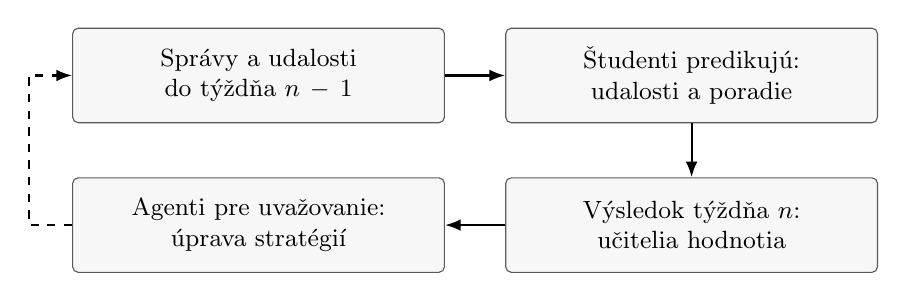
\begin{tikzpicture}
\node[box,text width=4.3cm,minimum height=1.2cm] (in) at (0,0) {Správy a udalosti\\do týždňa $n-1$};
\node[box,text width=4.3cm,minimum height=1.2cm] (pred) at (5.5,0) {Študenti predikujú:\\udalosti a poradie};
\node[box,text width=4.3cm,minimum height=1.2cm] (feedback) at (5.5,-1.9) {Výsledok týždňa $n$:\\učitelia hodnotia};
\node[box,text width=4.3cm,minimum height=1.2cm] (update) at (0,-1.9) {Agenti pre uvažovanie:\\úprava stratégií};
\draw[arr] (in)--(pred);
\draw[arr] (pred)--(feedback);
\draw[arr] (feedback)--(update);
\draw[arr,dashed] (update.west)--++(-0.55,0)|- (in.west);
\end{tikzpicture}
\caption{Cyklus MENTOR: predikcia týždňa $n$ a úprava stratégií pre ďalšie obdobie. Vlastné spracovanie podľa \mentorref{obr.~3 a algoritmus~1}.}
\label{fig:mentor}
\end{figure}


\subsection{Porovnanie a výsledky}
\begin{table}[H]
\centering
\caption{Porovnanie oboch metód. Vlastné spracovanie podľa \serref{kap.~2--3} a \mentorref{kap.~3--5}.}
\label{tab:comparison}
\small
\begin{tabularx}{\textwidth}{@{}p{2.35cm}YY@{}}
\toprule
Vlastnosť & SER & MENTOR\\
\midrule
Vstup & Články spojené s firmou a identifikátor jej akcie & Správy, známe udalosti a minulé výnosy odvetví\\
Výstup & Odhad výnosu akcie na ďalší deň alebo týždeň & Budúce udalosti a poradie odvetvových indexov\\
Úloha LLM & Získanie udalostí z textu a ich kontrola & Hľadanie a predikcia udalostí, hodnotenie chýb\\
Čo sa mení & Vektory, attention a MLP podľa chyby výnosu & Textové postupy podľa hodnotenia učiteľov\\
Overenie & Test na ďalšom roku, výsledky portfólií a regresie & Testy po týždňoch, zhoda udalostí, poradie a portfóliá\\
\bottomrule
\end{tabularx}
\end{table}

Autori testujú MENTOR na čínskych príspevkoch vplyvných autorov a na anglických finančných správach z rokov 2023--2024. Pri predikcii udalostí zisťujú, ktoré predikované udalosti sa zhodujú so skutočnými. Pri poradí odvetví používajú Spearmanovu koreláciu, Kendallov koeficient a zhodu odvetví na prvých miestach. Prvé dve metriky porovnávajú predikované poradie so skutočným \mentorref{kap.~5.1--5.2}. Tieto testy však neoverujú, či by napríklad predikcia pravdepodobnosti 70\,\% zodpovedala približne 70\,\% skutočných prípadov. To by bola samostatná kontrola kalibrácie pravdepodobností.

Na 11 odvetviach S\&P dosahuje MENTOR\_O1 Spearmanovu koreláciu 0,221. Metóda Momentum dosahuje 0,159. Pri zhode troch najvyšších odvetví sú výsledky 0,394 a 0,364. Na deviatich odvetviach A-share má MENTOR\_O1 koreláciu 0,173. Pri zhode prvých troch odvetví však dosahuje 0,439 oproti 0,444 pri Momentum. MENTOR teda nie je lepší vo všetkých ukazovateľoch \mentorref{tab.~3}.

Autori uvádzajú aj výsledky portfólií a skúšajú rôzne dvojice modelov učiteľ--študent \mentorref{kap.~5.6, tab.~5--6}. Tieto výnosy nemožno priamo porovnať s výsledkami SER. Články používajú iné obdobia, aktíva a testy. Niektoré presné definície metrík a vzory pokynov sú v samostatných prílohách MENTOR. Pri príprave tejto práce tieto prílohy neboli dostupné na overenie.

\FloatBarrier
\section{Návrh pre bakalársku prácu}
Táto časť opisuje môj návrh. Zo SER chcem využiť hlavne oddelenie dvoch úloh. Hotová LLM by spracovala text a menší učený model by predikoval výnos konkrétnej akcie. MENTOR ukazuje rozdiel medzi známymi a budúcimi udalosťami a použitie spätnej väzby po výsledku. Celý systém viacerých agentov však prvý prototyp nepotrebuje.

Vstupom by bol opis možnej udalosti, jej termín a vtedy dostupná pravdepodobnosť. Poskytol by ich externý zdroj, napríklad predikčný trh. LLM by pripravila štruktúrovaný záznam. Musela by zachovať podmienky, termín aj to, že udalosť ešte nemusí nastať. Prediktor by použil tento záznam, pravdepodobnosť a trhové údaje na odhad výnosu. Nové informácie by mohli zmeniť predikciu aj rozhodnutie o pozícii bez nového učenia. Vlastné vytváranie scenárov a ich pravdepodobností pomocou LLM zostáva možným rozšírením.

SER sa učí odhadovať výnos po zverejnení správy. Môj návrh sa týka očakávaní pred udalosťou. Model naučený na správach preto nemusí správne odhadnúť výnos pri konkrétnom budúcom scenári. Investori už môžu udalosť očakávať. Časť očakávania môže byť v cene a dôležitý môže byť rozdiel medzi očakávaním a skutočným výsledkom.

Tréningový príklad by preto obsahoval iba informácie dostupné v minulom okamihu rozhodnutia $t$: vtedajší opis, pravdepodobnosť $p_t$ a stav trhu. Cieľom by bol skutočný výnos od najskoršieho možného obchodu do konca zvoleného obdobia. Neskoršiu pravdepodobnosť, ktorá už pozná výsledok, nemožno použiť namiesto pôvodnej. Ani rozdelenie aktualizácií jednej udalosti medzi učenie a test nesmie prezradiť budúci výsledok.

Pravdepodobnosť udalosti nie je pravdepodobnosťou rastu akcie. Pre udalosť $A$, dostupné informácie $\mathcal I_t$ a $p_t=P(A\mid\mathcal I_t)$ platí
\begin{equation}
\mathbb E[r\mid\mathcal I_t]
=p_t\,\mathbb E[r\mid A,\mathcal I_t]
 +(1-p_t)\,\mathbb E[r\mid\neg A,\mathcal I_t].
\label{eq:expectation}
\end{equation}
Symbol $\mathbb E$ označuje očakávanú hodnotu. Prvá časť pravej strany opisuje výnos, keď udalosť nastane. Druhá opisuje výnos, keď nenastane. Obe časti majú váhu podľa pravdepodobnosti. Je to matematické vysvetlenie, nie vzorec prevzatý z článkov.

Napríklad pri pravdepodobnosti 0,6, očakávanom výnose $+4\,\%$ pri udalosti a $-2\,\%$ bez nej dostaneme $0{,}6\cdot4\,\%+0{,}4\cdot(-2\,\%)=1{,}6\,\%$. Ide iba o ilustračné čísla. Výpočet $0{,}6\cdot4\,\%$ by vynechal druhý prípad. Ak model už odhaduje celkový očakávaný výnos, netreba ho automaticky znovu násobiť pravdepodobnosťou. Externá pravdepodobnosť môže byť zle kalibrovaná. Ani odhad výnosu pri udalosti sám nedokazuje jej príčinný účinok.

Konkrétne udalosti, akcie, zdroj a dĺžka predikovaného obdobia ešte nie sú vybrané. Rozhodnutia Federálneho rezervného systému sú iba kandidátom na overenie údajov. Hotový spojený dataset, jeho dostatočná veľkosť ani úspešnosť prototypu zatiaľ nie sú potvrdené.

Na učenie treba použiť staršie údaje a na test novšie. Model chcem porovnať s jednoduchou metódou, ktorá používa iba ceny, a s verziami bez udalostí alebo pravdepodobností. Chybu veľkosti výnosu, správnosť smeru a výsledok obchodovania po nákladoch treba merať zvlášť.

\section{Záver}
V SER jazykový model získava udalosti zo správ. Ďalší model používa ich vektory, vektor akcie, attention a MLP na odhad výnosu. Výsledky sú sľubné, ale ich použitie v inej úlohe treba overiť. MENTOR predikuje aj budúce udalosti a mení textové stratégie agentov. Jeho finančným výstupom je poradie odvetví.

V bakalárskej práci najprv overím údaje o historických očakávaniach. Potom bude možné pripraviť príklady bez informácií z budúcnosti. Až experiment ukáže, či udalosti a ich pravdepodobnosti zlepšia predikciu oproti jednoduchším metódam.

\printbibliography[title={Literatúra}]
\end{document}
